\clearpage

\subsection{Translucent without Survivability}\label{ILP_Transluc_Survivability}
\begin{tcolorbox}	
\begin{tabular}{p{2.75cm} p{0.2cm} p{10.5cm}} 	
\textbf{Student Name}  &:& Tiago Esteves    (October 03, 2017 - )\\
\textbf{Goal}          &:& Implement the ILP model for the translucent transport mode without survivability.
\end{tabular}
\end{tcolorbox}

\subsubsection{Model description}

First, for a better understanding of the functions and variables used in the ILP, a table \ref{description_transluc} will be created with all indexes, inputs and variables and with their respective description.

\begin{table}[h!]
\centering
\begin{tabular}{ |p{1cm}||p{13cm}|}
 \hline
 \multicolumn{2}{|c|}{Description of notation used in the objective function} \\
 \hline
 \hline
 $i$ & index for start node of a physical link \\
 $j$ & index for end node of a physical link \\
 $o$ & index for node that is origin of a demand \\
 $d$ & index for node that is destination of a demand \\
 $c$ & index for bit rate of the client signal \\
 $($ i,j $)$ & physical link between the nodes $i$ and $j$ \\
 $($ o,d $)$ & demand between the nodes $o$ and $d$ \\
 $C$ & set of the client signal \\
 $L_{ij}$ & binary variable indicating if link between the nodes $i$ and $j$ is used \\
 $Ls_{ij}^{od}$ & Number of ODU-o low speed signals from node $o$ to node $d$ employing lightpath ($i$,$j$) \\
 $f_{ij}^{od}$ & Number of 100 Gbit/s optical channels (number of flows) between the link $i$ and $j$ for all demand pairs between $o$ and $d$ \\
 $\lambda_{od}$ & Number of lightpath channels between the nodes $o$ and $d$ \\
 $B$ & Client signals granularities $($1.25, 2.5, 10, 40, 100$)$ \\
 $D_{odc}$ & Client traffic demands between the nodes $o$ and $d$ with bit rate $c$ \\
 $G$ & Network topology in form of adjacency matrix \\
 \hline
\end{tabular}
\caption{Table with description of variables}
\label{description_transluc}
\end{table}

Before carrying out the description of the objective function we must take into account the following particularity of this mode of transport:
\begin{itemize}
  \item $N_{OXC,n}$ = 1, \quad $\forall$ n that process traffic
  \item $N_{EXC,n}$ = 1, \quad $\forall$ n that process traffic
\end{itemize}

\vspace{7pt}
The objective function of following the ILP is a minimization of the CAPEX through the equation \ref{Capex} where in this case for the cost of nodes we have in consideration electric \ref{Capex_Node_EXC} and optical cost \ref{Capex_Node_OXC}. In this case the value of $P_{exc,c,n}$ is obtained by equation \ref{EXC_pexc1_transluc} for short-reach and by the equation \ref{EXC_pexc2_transluc} for long-reach and the value of $P_{oxc,n}$ is obtained by equation \ref{OXC_poxc_transluc}.\\

The equation \ref{EXC_pexc1_transluc} refers to the number of sort-reach ports of the electrical switch with bit-rate $c$ in node $n$, $P_{exc,c,n}$, i.e. the number of tributary ports with bit-rate $c$ in node $n$ which can be calculated as

\begin{equation}
P_{exc,c,n} = \sum_{d=1}^{N} D_{nd,c}
\label{EXC_pexc1_transluc}
\end{equation}

\vspace{11pt}
\noindent
where $D_{nd,c}$ are the client demands between nodes $n$ and $d$ with bit rate $c$.\\

In this case there is the following particularity:
\begin{itemize}
  \item When $n$=$d$ the value of client demands is always zero, i.e, $D_{nn,c}=0$
\end{itemize}

\vspace{11pt}
As previously mentioned, the equation \ref{EXC_pexc2_transluc} refers to the number of long-reach ports of the electrical switch with bit-rate -1 in node n, $P_{exc,-1,n}$, i.e. the number of add ports of node n which can be calculated as

\begin{equation}
P_{exc,-1,n} = \sum_{j=1}^{N} \lambda_{nj}
\label{EXC_pexc2_transluc}
\end{equation}

\vspace{11pt}
\noindent
where $\lambda_{nj}$ is the number of optical channels between node $n$ and node $j$.\\

The equation \ref{OXC_poxc_transluc} refers to the number of ports in optical switch in node n, $P_{oxc,n}$, i.e. the number of line ports and the number of adding ports of node n which can be calculated as

\begin{equation}
P_{oxc,n} = \sum_{j=1}^{N} f_{nj}^{od} + \sum_{j=1}^{N} \lambda_{nj}
\label{OXC_poxc_transluc}
\end{equation}

\vspace{11pt}
\noindent
where $f_{nj}^{od}$ refers to the number of line ports for all demand pairs (od) and $\lambda_{nj}$ refers to the number of add ports.\\

The objective function, to be minimized, is the expression \ref{ILPOpaque_CAPEX}, i.e.,
\begin{equation*}
  minimize \qquad \Big\{ \quad C_C \quad \Big\}
\end{equation*}

$subject$ $to$
\begin{equation}
\sum_{j\textbackslash \{o\}} Ls_{ij}^{odc} = D_{odc}  \qquad \qquad \qquad \qquad \qquad \qquad \qquad \qquad \qquad
\forall(o,d) : o < d, \forall i: i = o
\label{ILPTransluc1}
\end{equation}

This constraint are the virtual flow conservation constraints and ensure that, for all (o,d) pairs with bit rate $c$ we routes demand traffic of flow from node $o$ to node $d$ with bit rate $c$ for all bidirectional links (i,j) when $j$ is not equal to the origin of the demand.

\begin{equation}
\sum_{j\textbackslash \{i,o\}} Ls_{ij}^{odc} = \sum_{j\textbackslash \{i,d\}} Ls_{ji}^{odc} \qquad \qquad \qquad \qquad \qquad \qquad \qquad
\forall(o,d) : o < d, \forall i: i \neq o,d
\label{ILPTransluc2}
\end{equation}

In this constraint, assuming bidirectional traffic, so the demand traffic of flow in both directions of the link is the same.

\begin{equation}
\sum_{j\textbackslash \{d\}} Ls_{ji}^{odc} = D_{odc} \qquad \qquad \qquad \qquad \qquad \qquad \qquad \qquad \qquad
\forall(o,d) : o < d, \forall i: i = d
\label{ILPTransluc3}
\end{equation}

This constraint are the virtual flow conservation constraints and ensure that, for all (o,d) pairs with bit rate $c$ we routes demand traffic of flow from node $o$ to node $d$ with bit rate $c$ for all bidirectional links (j,i) when $i$ is not equal to the destination of the demand.

\begin{equation}
\sum_{o=1} \sum_{d=o+1} B(c) Ls_{ij}^{odc} \leq  \tau \lambda_{od} \qquad \qquad \qquad \qquad \qquad \qquad \qquad \qquad \qquad \qquad
\forall (i,j)
\label{ILPTransluc4}
\end{equation}

This restriction is considered grooming constraint and the variable $\tau$ is always 100 Gbits/s.

\begin{equation}
\sum_{j\textbackslash \{o\}} f_{ij}^{od} = \lambda_{od}  \qquad \qquad \qquad \qquad \qquad \qquad \qquad \qquad \qquad
\forall(o,d) : o < d, \forall i: i = o
\label{ILPTransluc6}
\end{equation}

This constraint are equal to the constraint \ref{ILPOpaque1_CAPEX} assuming that Z variable has the value of number of optical channels between this demand for all bidirectional links.

\begin{equation}
\sum_{j\textbackslash \{o\}} f_{ij}^{od} = \sum_{j\textbackslash \{d\}} f_{ji}^{od} \qquad \qquad \qquad \qquad \qquad \qquad \qquad \qquad
\forall(o,d) : o < d, \forall i: i \neq o,d
\label{ILPTransluc7}
\end{equation}

This constraint are equal to the constraint \ref{ILPOpaque2_CAPEX}.

\begin{equation}
\sum_{j\textbackslash \{d\}} f_{ji}^{od} = \lambda_{od}  \qquad \qquad \qquad \qquad \qquad \qquad \qquad \qquad \qquad
\forall(o,d) : o < d, \forall i: i = d
\label{ILPTransluc8}
\end{equation}

This constraint are equal to the constraint \ref{ILPOpaque3_CAPEX} assuming that Z variable has the value of number of optical channels between this demand for all bidirectional links.

\begin{equation}
\sum_{o=1} \sum_{d=o+1} \left( f_{ij}^{od} + f_{ji}^{od}\right) \leq K_{ij} G_{ij} L_{ij} \qquad \qquad \qquad \qquad \qquad \qquad \qquad
\forall (i,j) : i < j
\label{ILPTransluc9}
\end{equation}

This restriction answers capacity constraint problem. Then, total flows must be less or equal to the capacity of network links. For any situation the maximum number of optical channels supported by each transmission system is 100, i.e., $K_{ij}$ = 100.

\begin{equation}
f_{ij}^{od} , f_{ji}^{od} , Ls_{ij}^{odc} , Ls_{ji}^{odc} , \lambda_{od} \in \mathbb{N}   \qquad \qquad \qquad \qquad \qquad
\forall(i,j) : i < j, \forall(o,d) : o < d
\label{ILPTransluc10}
\end{equation}

This constraint defines that these variables must be a counting number.

\begin{equation}
L_{i,j} \in \{0,1\} \qquad \qquad \qquad \qquad \qquad \qquad \qquad \qquad \qquad \qquad \qquad \qquad \qquad \qquad
\forall(i,j)
\label{ILPTransluc11}
\end{equation}

Last constraint refers to the use of the link where this variable can be zero if it is not being used or one if is being used.

\subsubsection{Result description}

To perform the calculations using the implementation of the models described previously it is necessary to use a mathematical software tool. For this we will use MATLAB which is ideal for dealing with linear programming problems and can call the LPsolve through an external interface.
We already have all the necessary to obtain the CAPEX value for the reference network \ref{Reference_Network_Topology}. As described in the subsection of network traffic \ref{Reference_Network_Traffic}, we have three values of network traffic so we have to obtain three different CAPEX. The value of the CAPEX of the network will be calculated based on the costs of the equipment present in the table \ref{table_cost_ilp}.\\

\textbf{Low Traffic Scenario:}\\

In this scenario we have to take into account the traffic calculated in \ref{low_scenario}. In a first phase we will show the various existing topologies of the network. The first are the allowed topologies, physical and optical topology, the second are the logical topology for all ODUs and finally the resulting physical and optical topology.

\begin{figure}[h!]
\centering
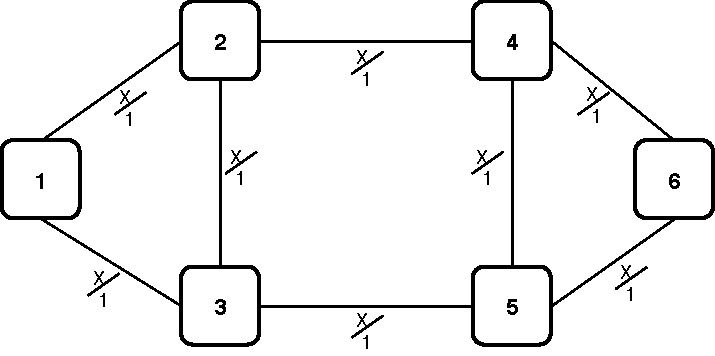
\includegraphics[width=11cm]{sdf/ilp/translucent_survivability/figures/allowed_physical_topology}
\caption{Allowed physical topology. The allowed physical topology is defined by the duct and sites in the field. It is assumed that each duct supports up to 1 bidirectional transmission system and each site supports up to 1 node.}
\label{allowed3_physical_low}
\end{figure}

\newpage
\begin{figure}[h!]
\centering
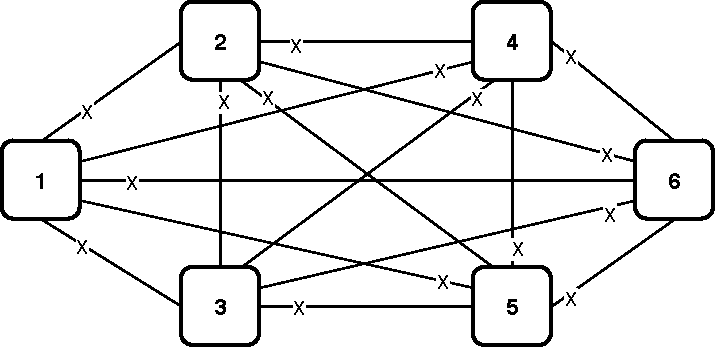
\includegraphics[width=11cm]{sdf/ilp/translucent_survivability/figures/allowed_optical_topology}
\caption{Allowed optical topology. The allowed optical topology is defined by the transport mode (translucent transport mode in this case). It is assumed that each connections between demands supports up to 100 lightpaths.}
\label{allowed3_optical_low}
\end{figure}

\begin{figure}[h!]
\centering
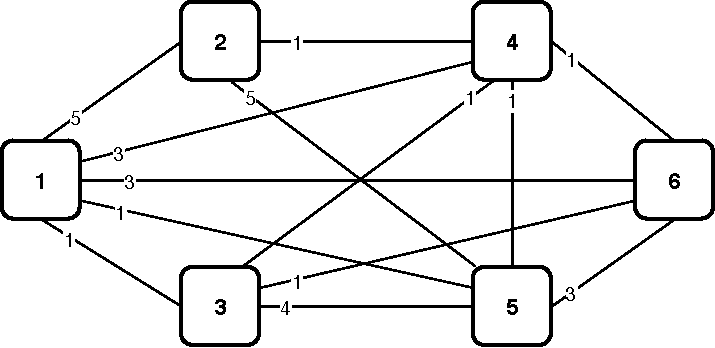
\includegraphics[width=11cm]{sdf/ilp/translucent_survivability/figures/logical_topology_ODU0_low}
\caption{ODU0 logical topology defined by the ODU0 traffic matrix.}
\label{logical3_ODU0_low}
\end{figure}

\begin{figure}[h!]
\centering
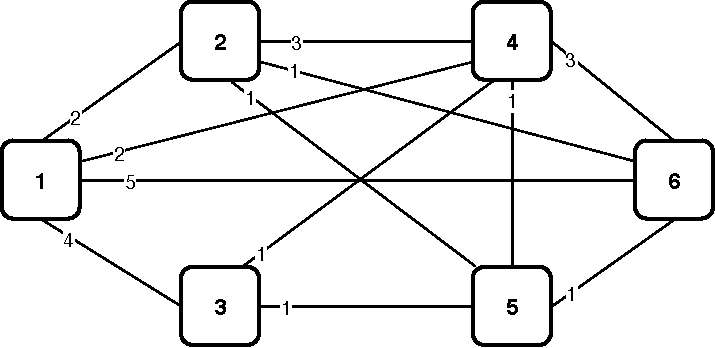
\includegraphics[width=11cm]{sdf/ilp/translucent_survivability/figures/logical_topology_ODU1_low}
\caption{ODU1 logical topology defined by the ODU1 traffic matrix.}
\label{logical3_ODU1_low}
\end{figure}

\newpage
\begin{figure}[h!]
\centering
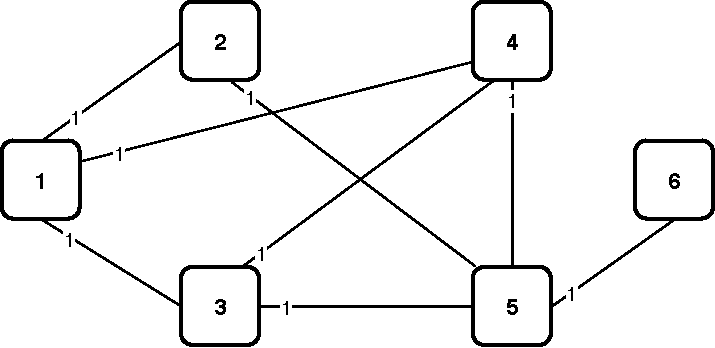
\includegraphics[width=12cm]{sdf/ilp/translucent_survivability/figures/logical_topology_ODU2_low}
\caption{ODU2 logical topology defined by the ODU2 traffic matrix.}
\label{logical3_ODU2_low}
\end{figure}

\begin{figure}[h!]
\centering
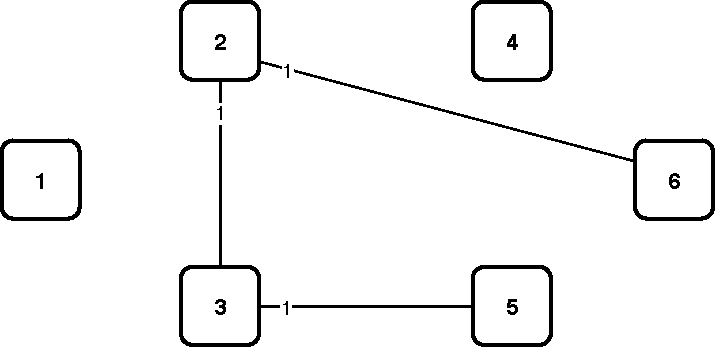
\includegraphics[width=12cm]{sdf/ilp/translucent_survivability/figures/logical_topology_ODU3_low}
\caption{ODU3 logical topology defined by the ODU3 traffic matrix.}
\label{logical3_ODU3_low}
\end{figure}

\begin{figure}[h!]
\centering
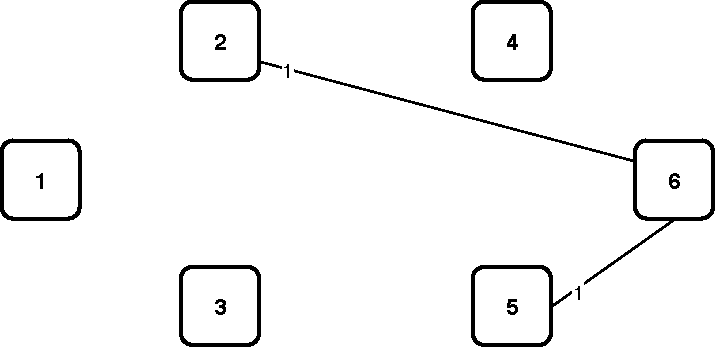
\includegraphics[width=12cm]{sdf/ilp/translucent_survivability/figures/logical_topology_ODU4_low}
\caption{ODU4 logical topology defined by the ODU4 traffic matrix.}
\label{logical3_ODU4_low}
\end{figure}
\newpage
\begin{figure}[h!]
\centering
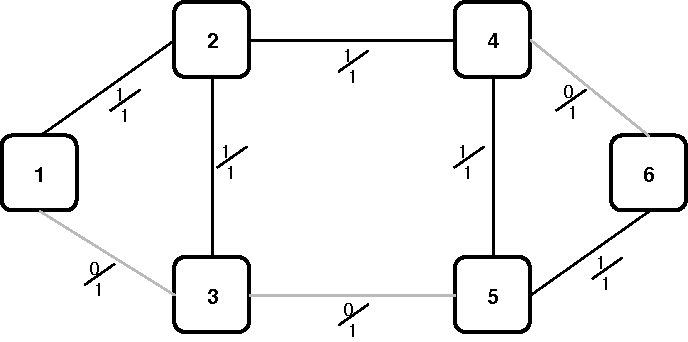
\includegraphics[width=12cm]{sdf/ilp/translucent_survivability/figures/physical_topology_low}
\caption{Physical topology after dimensioning.}
\label{physical3_low}
\end{figure}

\begin{figure}[h!]
\centering
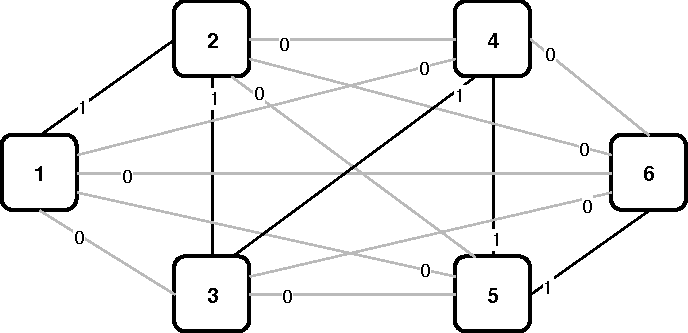
\includegraphics[width=12cm]{sdf/ilp/translucent_survivability/figures/optical_topology_low}
\caption{Optical topology after dimensioning.}
\label{optical3_low}
\end{figure}

In table \ref{link_transluc_surv_ref_low} we can see the number of optical channels calculated using \ref{Capex_Link} and \ref{ILPOpaque_CAPEX} and the number of amplifiers for each link calculated using \ref{Capex_amplifiers}. In the case where there are no optical channels we assume that the number of amplifiers is zero.\\

In table \ref{node_transluc_surv_ref_low} we can see the resulting nodal degree at the physical layer, calculated based on the number of connections that the node in question performs, the number of line ports and add ports using \ref{OXC_poxc_transluc} the number of long-reach transponders using \ref{EXC_pexc2_transluc} and the number of tributary ports using \ref{EXC_pexc1_transluc}.\\
\newpage
\begin{table}[h!]
\centering
\begin{tabular}{|| c | c | c ||}
 \hline
 \multicolumn{3}{|| c ||}{Information regarding links} \\
 \hline
 \hline
 Bidirectional Link & Optical Channels & Amplifiers\\
 \hline
 Node 1 <-> Node 2 & 8 & 4 \\
 Node 1 <-> Node 3 & 0 & 0 \\
 Node 2 <-> Node 3 & 6 & 0 \\
 Node 2 <-> Node 4 & 2 & 6 \\
 Node 3 <-> Node 5 & 1 & 8 \\
 Node 4 <-> Node 5 & 3 & 1 \\
 Node 4 <-> Node 6 & 0 & 0 \\
 Node 5 <-> Node 6 & 2 & 3 \\
 \hline
\end{tabular}
\caption{Table with information regarding links for translucent mode without survivability.}
\label{link_transluc_surv_ref_low}
\end{table}

\vspace{17pt}
\begin{table}[h!]
\centering
\begin{tabular}{|| c | c | c | c | c | c ||}
 \hline
 \multicolumn{6}{|| c ||}{Information regarding nodes} \\
 \hline
 \hline
 \multicolumn{2}{|| c |}{ } & \multicolumn{2}{ c |}{Electrical part} & \multicolumn{2}{ c ||}{Optical part} \\
 \hline
 Node & Resulting Nodal Degree & Tributary Ports & LR Transponders & Add Ports & Line Ports\\
 \hline
 1 & 1 & 29 & 8 & 8 & 8 \\
 2 & 3 & 23 & 12 & 12 & 16 \\
 3 & 2 & 18 & 7 & 7 & 7 \\
 4 & 2 & 20 & 5 & 5 & 5 \\
 5 & 3 & 24 & 6 & 6 & 6 \\
 6 & 1 & 22 & 2 & 2 & 2 \\
\hline
\end{tabular}
\caption{Table with information regarding nodes for translucent mode without survivability.}
\label{node_transluc_surv_ref_low}
\end{table}

\vspace{17pt}
Through the information obtained previously on the nodes we can now create tables with detailed information about each node. In each table mentioned below we can see how many ports are connected to a given node and its bit rate (in relation to the line ports) and how many ports are assigned to each different bit rate (in relation to the tributary ports).\\
